\documentclass{article}
\usepackage[utf8]{inputenc}
\usepackage{hyperref}
\usepackage{authblk}
\usepackage{listings}

\title{TKG Automation with Cloud Assembly}
\author{Assaf Sauer, Tim Gretler}
\affil{Vmware Inc.}
\date{May 2020}

\usepackage{natbib}
\usepackage{graphicx}

\begin{document}



\maketitle


\newpage
\tableofcontents
\newpage


\section{Introduction}
This is a Guide on how to automate Tanzu Kubernetes Grid with Cloud Assembly and integrate it with Tanzu Mission Control, which is part of the VMware modern application portfolio \citep{tanzu}. It is thought to be a proof of concept to show how you can automate the control plane creation of Tanzu Kubernetes Grid. This will give you the ability to deploy a TKG management plane with a few clicks on AWS and vSphere. 

\subsection{Tanzu Kubernetes Grid}
Tanzu Kuberenetes Grid is a certified Kubernetes distribution developed by VMware \citep{tkg}. It strives to build a simplified infrastructure across a multi-cloud environment. This will improve ease of development and also the speed of development, while still providing production-grade stability. New automation capabilities provide a much faster and easier setup and therefore higher flexibility in a diverse working environment. 

\subsection{Cloud Assembly}
Cloud Assembly is a VMware automation product \citep{cloudassembly}. It gives you a simple interface to your multi-cloud environment. With Cloud Assembly you have Infrastructure-as-Code and you can deploy templates to multiple cloud from a single interface. This provides the benefit of single source of truth for your deployments independent of the underlying cloud. 


\subsection{Tanzu Mission Control}
Tanzu Mission Control is the central control hub for your Kubernetes clusters \citep{tmc}. Tanzu Mission Control gives you insights into your fleet of clusters. One can also apply policies across all clusters from Tanzu Mission Control. You can attach any CNCF certified cluster and manage its lifecycle.


\newpage

\section{Manual}
\subsection{Prerequisites}
\begin{itemize}
  \item Access to Cloud Assembly
  \item vSphere Environment 
  \item AWS Account
\end{itemize}

\subsection{General Overview}

\begin{figure}[h!]
\centering
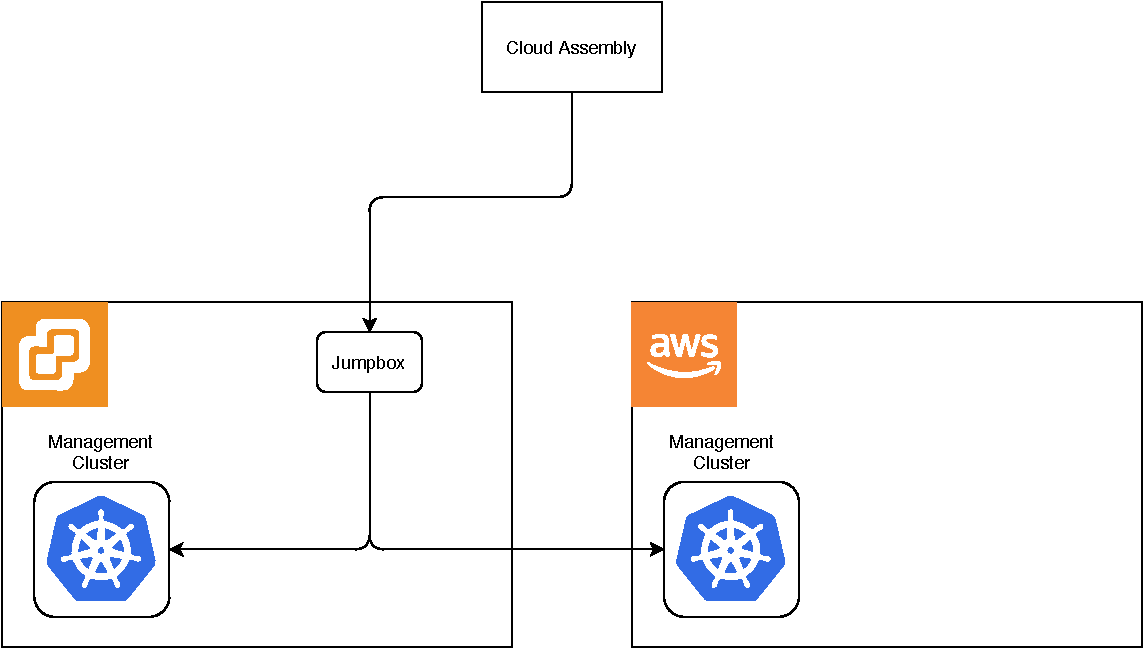
\includegraphics[scale=0.6]{figures/overview-mc.pdf}
\caption{Architecture created by automation}
\label{fig:arch}
\end{figure}

Figure \ref{fig:arch} provides an illustration of the created architecture by the automation. Cloud Assembly will deploy a Virtual Machine inside your vCenter and install all the software needed for TKG. After the software installation, it automatically deploys a management cluster to vSphere and AWS. When the process is complete you will have access to both management clusters and you are able to create clusters as you wish 


\subsection{Setup Cloud Assembly}

Instructions to setup Cloud Assembly with vCenter. Follow all steps. This guide assumes that you have no configurations in cloud assembly. You can skip certain steps if you already have a working setup. 

\subsubsection{Connect Cloud Assembly and vCenter}
\begin{enumerate}
  \item Log into Cloud Assembly
  \item Switch to infrastructure tab of Cloud Assembly
  \item In the menu on the left choose Cloud Accounts
  \item Click "Add Account" and choose vCenter
  \item Click "New Cloud Proxy" and deploy a proxy by following the given instruction if you haven't already 
  \item Name your Cloud Account and provide login credentials of your vCenter
  \item Click add at the bottom
\end{enumerate}


\subsubsection{Add Cloud Zone}
\begin{enumerate}
  \item Log into Cloud Assembly
  \item Switch to infrastructure tab of Cloud Assembly
  \item In the menu on the left choose Cloud Zones
  \item If you have correctly setup the vCenter connection you should see your vCenter under Account/Region. Choose your vCenter
  \item Name your Cloud Zone and add it
\end{enumerate}

\subsubsection{Create Ubuntu 18.04 Template in vCenter}

\begin{enumerate}
  \item Log into your vCenter
  \item Right Click on your Datacenter and select "Deploy OVF Template"
  \item As source you can add following url \url{https://cloud-images.ubuntu.com/bionic/current/bionic-server-cloudimg-amd64.ova} . This will get you the ubuntu cloud image
  \item You can just click through the remaining options
  \item Click "Finish"
  \item Wait until you see Ubuntu ova deployed to your vCenter
  \item Right Click on the deployed VM -> choose "Template" -> click convert to Template
  \item Now you should see a Ubuntu template under your templates
\end{enumerate}


\subsubsection{Add Image mapping}

\begin{enumerate}
  \item Log into Cloud Assembly
  \item Switch to infrastructure tab of Cloud Assembly
  \item In the menu on the left choose Image Mapping
  \item Click "New Image Mapping"
  \item Name it "tkg-template"
  \item Select your Account/Region
  \item If you correctly created the Ubuntu template you should now see it under Image. Select it!
  \item Click create
\end{enumerate}

\subsubsection{Add Flavor mapping}

\begin{enumerate}
  \item Log into Cloud Assembly
  \item Switch to infrastructure tab of Cloud Assembly
  \item In the menu on the left choose Flavor Mapping
  \item Click "New Flavor Mapping" if a small Mapping doesn't already exist. If it already exists make sure you have a mapping for your account!
  \item Name it "small"
  \item Select your Account/Region
  \item Configure your small Flavor by choosing an appropriate number of CPU and Memory
  \item Click create
\end{enumerate}


\subsubsection{Create Project}

\begin{enumerate}
  \item Log into Cloud Assembly
  \item Switch to infrastructure tab of Cloud Assembly
  \item In the menu on the left choose Projects
  \item Click "New Project"
  \item Name the project
  \item Switch tab to "user" and add yourself
  \item Switch tab to "provisioning" and add your cloud zone
  \item Click create
\end{enumerate}

\subsection{Create Tanzu Mission Control API Keys} \label{tmctoken}

\begin{enumerate}
  \item Log into VMware Cloud Services
  \item Click on your name on the top right and choose "My Account"
  \item Switch to tab API Tokens
  \item Click "Generate Token"
  \item Name the token and choose "All Roles"
  \item Generate Token and save it!
\end{enumerate}

\subsection{Deploy Tanzu Kubernetes Grid}

Now we have everything setup to deploy TKG. As an attachment to this PDF you will find the Cloud Assembly template, which deploys TKG. You will also get AWS credentials to download the TKG binaries. You should keep them secret and don't publish them anywhere!


\subsubsection{Import Template to Cloud Assembly}

\begin{enumerate}
  \item Log into Cloud Assembly
  \item Switch to Design tab of Cloud Assembly
  \item Click "Upload" 
  \item Name your design, select your project and upload the attached TKG deployment yaml.
  \item Click "Upload" 
\end{enumerate}


\subsubsection{Deploy TKG}

\begin{enumerate}
  \item Log into Cloud Assembly
  \item Switch to Design tab of Cloud Assembly
  \item Go to your design by selecting it
  \item Click "Deploy" on the bottom left
  \item Name your Deployment and choose current draft
  \item Fill out prompted values
  \begin{itemize}
  \item \verb|AWS_KEY_ID_S3:| ID of provided credentials to download binaries
  \item \verb|AWS_SECRET_KEY_S3:| Secret Key of provided credentials to download binaries
  \item \verb|AWS_KEY_ID_COMPUTE:| Key ID of your AWS account on where to deploy TKG. Need to have administrator permissions
  \item \verb|AWS_SECRET_KEY_COMPUTE:| Secret Key of your AWS account on where to deploy TKG
  \item \verb|AWS_COMPUTE_REGION:| Region where to deploy
  \item \verb|TMC_API_TOKEN:| Tanzu Mission Control Token created in \ref{tmctoken}
  \item \verb|tkg-cli:| Name of tkg-cli file in s3. Can be left default
  \item \verb|haproxy-ova:| Name of haproxy-ova file in s3. Can be left default
  \item \verb|tkg-ova:| Name of tkg-ova file in s3. Can be left default
  \item \verb|datastore:| Datastore to use
  \item \verb|vcenterIP:| IP of your vCenter
  \item \verb|vcenterUser:| User of your vCenter
  \item \verb|vcenterPassword:| Password of your vCenter
  \item \verb|resourcePool:| Resourcepool to deploy to
  \item \verb|sshKey:| Public Key to connect to TKG nodes

\end{itemize}
\end{enumerate}

\noindent {\bf Note:} If you don't want to deploy to AWS/vSphere you can fill in an invalid value. This leads to not deploying this provider. The same goes for TMC.
\\

\noindent Now you can see your deployment under the Cloud Assembly tab Deployments. You will see the IP of your newly created jumpbox. You can now connect to the jumpbox, but the TKG installation wil take aprox. 45-60min.



\section{Tanzu Kubernets Grid Basics}

Interaction with TKG happens through the command line. This sections provides a brief overview.
TKG uses the cluster API \citep{clusterapi} to create new clusters therefore you need a seperate management cluster for vCenter and AWS. In general you always have to set a context, which is either the vCenter or the AWS management cluster. \\

\subsection{General Help}

The command line interface is easy to use if you are familiar with the linux command line. If you don't know what to type you can always call for help like this:

\begin{lstlisting}
  $ tkg -h
\end{lstlisting}

or 

\begin{lstlisting}
  $ tkg <command> -h
\end{lstlisting}




\subsection{Some TKG CLI commands}

\noindent This command sets the management cluster. You can switch between management clusters as you like.
\begin{lstlisting}
  $ tkg set management-cluster <cluster_name> 
\end{lstlisting}


\noindent This command lets you create a new cluster.
\begin{lstlisting}
  $ tkg create cluster <new_cluster_name>
\end{lstlisting}





\section{Troubleshooting}

\subsection{Debugging Jumpbox}

Access cloud-init logs:
\begin{lstlisting}[language=bash]
  $ cat /var/log/cloud-init-output.log
\end{lstlisting}

\subsection{Cloud Assembly Deployment failed}
To debug cloud assembly following steps are helpful. 

\begin{enumerate}
  \item Log into Cloud Assembly
  \item Go to Cloud Assembly tab Infrastructure
  \item In the panel on the left hand side choose "Requests" under "Activity"
  \item Now you can find your deployment that failed
  \item You now see the decision steps of Cloud Assembly including where it failed
\end{enumerate}



\section{Appendix}

\subsection{Cloud-init}

Cloud init is a tool for customising cloud instances \citep{cloudinit}. It automatically applies user data to each cloud instance. It supports all major linux distributions and all major public and private cloud providers. In this automation we heavily used cloud init to configure the jumpbox, which is created by Cloud Assembly. Cloud Assembly provides you the possibility to use cloud init, that allowed us to run the entire setup of the management clusters in cloud init. 




\bibliographystyle{plain}
\bibliography{references}
\end{document}
